%%%%%%%%%%%%%%%%%%%%%%%%%%%%%%%%%%%%%%%%%
% Beamer Presentation
% LaTeX Template
% Version 1.0 (10/11/12)
%
% This template has been downloaded from:
% http://www.LaTeXTemplates.com
%
% License:
% CC BY-NC-SA 3.0 (http://creativecommons.org/licenses/by-nc-sa/3.0/)
%
%%%%%%%%%%%%%%%%%%%%%%%%%%%%%%%%%%%%%%%%%

%----------------------------------------------------------------------------------------
%	PACKAGES AND THEMES
%----------------------------------------------------------------------------------------

\documentclass{beamer}

\mode<presentation> {

% The Beamer class comes with a number of default slide themes
% which change the colors and layouts of slides. Below this is a list
% of all the themes, uncomment each in turn to see what they look like.

%\usetheme{default}
%\usetheme{AnnArbor}
%\usetheme{Antibes}
%\usetheme{Bergen}
%\usetheme{Berkeley}
%\usetheme{Berlin}
%\usetheme{Boadilla}
%\usetheme{CambridgeUS}
%\usetheme{Copenhagen}
%\usetheme{Darmstadt}
%\usetheme{Dresden}
%\usetheme{Frankfurt}
%\usetheme{Goettingen}
%\usetheme{Hannover}
%\usetheme{Ilmenau}
%\usetheme{JuanLesPins}
%\usetheme{Luebeck}
\usetheme{Madrid}
%\usetheme{Malmoe}
%\usetheme{Marburg}
%\usetheme{Montpellier}
%\usetheme{PaloAlto}
%\usetheme{Pittsburgh}
%\usetheme{Rochester}
%\usetheme{Singapore}
%\usetheme{Szeged}
%\usetheme{Warsaw}

% As well as themes, the Beamer class has a number of color themes
% for any slide theme. Uncomment each of these in turn to see how it
% changes the colors of your current slide theme.

%\usecolortheme{albatross}
%\usecolortheme{beaver}
%\usecolortheme{beetle}
%\usecolortheme{crane}
%\usecolortheme{dolphin}
%\usecolortheme{dove}
%\usecolortheme{fly}
%\usecolortheme{lily}
%\usecolortheme{orchid}
%\usecolortheme{rose}
%\usecolortheme{seagull}
%\usecolortheme{seahorse}
%\usecolortheme{whale}
%\usecolortheme{wolverine}

%\setbeamertemplate{footline} % To remove the footer line in all slides uncomment this line
%\setbeamertemplate{footline}[page number] % To replace the footer line in all slides with a simple slide count uncomment this line

\setbeamertemplate{navigation symbols}{} % To remove the navigation symbols from the bottom of all slides uncomment this line
}

\usepackage{graphicx} % Allows including images
\usepackage{booktabs} % Allows the use of \toprule, \midrule and \bottomrule in tables
\usepackage{hyperref}

%----------------------------------------------------------------------------------------
%	TITLE PAGE
%----------------------------------------------------------------------------------------

\title[ESKF Introduction]{Introduction to the Error-state Kalman filter} % The short title appears at the bottom of every slide, the full title is only on the title page

\author{Martin Brandt} % Your name
\date{\today} % Date, can be changed to a custom date

\begin{document}

\begin{frame}
\titlepage % Print the title page as the first slide
\end{frame}

\begin{frame}
\frametitle{Overview} % Table of contents slide, comment this block out to remove it
\tableofcontents % Throughout your presentation, if you choose to use \section{} and \subsection{} commands, these will automatically be printed on this slide as an overview of your presentation
\end{frame}

%----------------------------------------------------------------------------------------
%	PRESENTATION SLIDES
%----------------------------------------------------------------------------------------
\section{Motivation}

\begin{frame}
    \frametitle{Motivation}
    \begin{figure}
    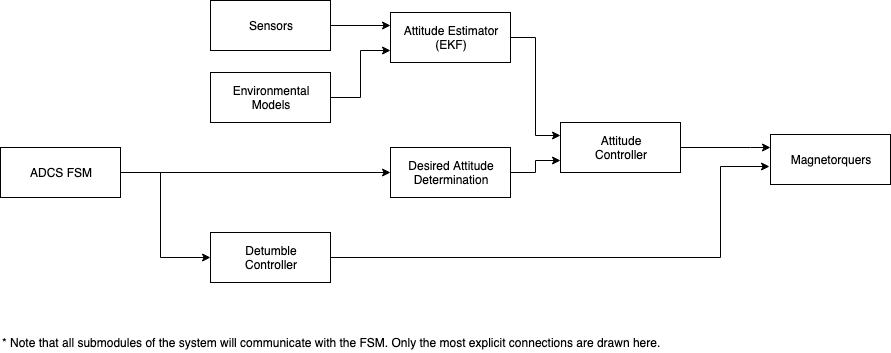
\includegraphics[width=0.8\linewidth]{adcs.png}
    \end{figure}
    The controller needs to know the attitude in order to control it, but there is no way to measure it directly $\rightarrow$ we have to estimate it!
\end{frame}

%------------------------------------------------

\begin{frame}
    \frametitle{Warning}
    These slides summarize A LOT of stuff, so you will probably not understand everything. But hopefully you will understand somewhat what the Kalman filter is and the reasoning behind the steps to why we use the error-state Kalman filter. This should also serve as an introduction and reference for new adcs people that wants to get into the ESKF. 
\end{frame}

%------------------------------------------------

\section{State space models}

\begin{frame}
    \frametitle{State space models}
    Want to represent an arbitrary system of differential equations in vector form. In general: $\dot{x} = f(x, u)$

    \begin{block}{Continous LTI state space model}
        \begin{equation}
        \begin{aligned}
            \dot{x} &= A x + B u \\
            y &=C x + D u
        \end{aligned}
        \end{equation}
    \end{block}

    \begin{block}{Discrete LTI state space model}
        \begin{equation}
        \begin{aligned}
            x[k+1] &= A x[k] + B u[k] \\
            y[k] &= C x[k] + D u[k]
        \end{aligned}
        \end{equation}
    \end{block}
\end{frame}

%------------------------------------------------

\begin{frame}
    \frametitle{Mass-spring-damper example}

    \begin{block}{How you are used to seeing it}
        \begin{equation}
            m \ddot{x}+d \dot{x} + ky=u
        \end{equation}
    \end{block}

    \begin{block}{State space representation}
        \begin{equation}
        \left[\begin{array}{c}{{\dot{x_1}}} \\ {\dot{x_2}}\end{array}\right] =\left[\begin{array}{cc}{0} & {1} \\ {-\frac{k}{m}} & {-\frac{d}{m}}\end{array}\right] \left[\begin{array}{c}{{x_1}} \\ {x_2}\end{array}\right] +\left[\begin{array}{c}{0} \\ {\frac{1}{m}}\end{array}\right] u
        \end{equation}
    \end{block}
\end{frame}

%------------------------------------------------

\section{The Kalman filter}

\begin{frame}
    \frametitle{Luenberger observer}
    Let's say we have a state space model of our system. How would we try to estimate the states of the system? 

    \begin{block}{The logical first try (open-loop observer)}
        \begin{equation}
            \dot{\hat{x}} = A \hat{x} + B u 
        \end{equation}
    \end{block}

    But because of modeling uncertainty our estimate will quickly diverge from the real value $\rightarrow$ include a correction term based on measurements (closing the loop) $\rightarrow$ Luenberger observer

    \begin{block}{The Luenberger observer}
        \begin{equation}
            \dot{\hat{x}} = A \hat{x} + B u + L (y - \hat{y}), \quad \hat{y} = C \hat{x}
        \end{equation}
    \end{block}
    But how do we decide the gain $L$?
\end{frame}

%------------------------------------------------

\begin{frame}
    \frametitle{The Kalman filter}
    Let us first assume that our process model and measurement model includes \textbf{normally distributed} noise:
    \begin{block}{Stochastic LTI system}
        \begin{equation}
            \begin{aligned}
                \dot{x} &= A x + B u + w \\
                y &=C x + D u + v
            \end{aligned}
        \end{equation}
    \end{block}
    The Kalman Filter is the optimal Luenberger observer for this system, in the sense that it minimizes \textbf{mean squared error}, i.e. $E\{(x-\hat{x})^2\}$. 
\end{frame}

%------------------------------------------------

\begin{frame}
    \frametitle{The Kalman filter equations}
    For the discrete case (which is what you would implement on a microcontroller) the Kalman filter equations are:
    \begin{figure}
        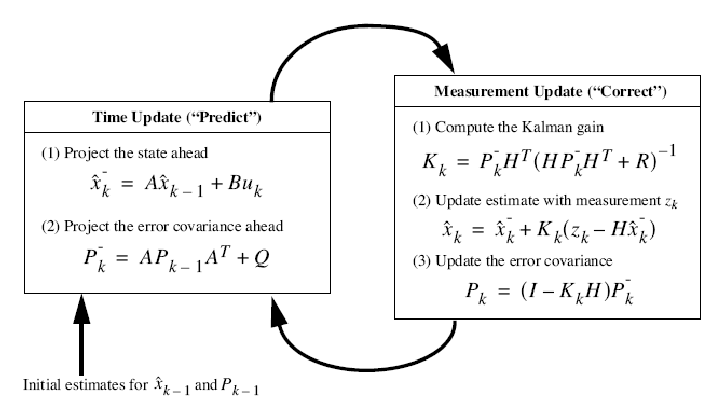
\includegraphics[width=0.8\linewidth]{kf_equations.png}
    \end{figure}
    The details are not important here, but note the predict + correct steps. 
\end{frame}

%------------------------------------------------

\begin{frame}
    \frametitle{The satellite kinematics and kinetics}
    Let's try to apply the Kalman filter to our satellite:
    \begin{block}{Satellite kinematics}
        \begin{equation}
            \begin{aligned}
                \dot{\mathbf{q}}=\frac{1}{2} \mathbf{q} \otimes \boldsymbol{\omega}
            \end{aligned}
        \end{equation}
    \end{block}
    \begin{block}{Satellite kinetics}
        \begin{equation}
            \begin{aligned}
                \dot{\omega}=J^{-1}\left[\mathbf{L}-\omega \times\left(J \omega\right)\right]
            \end{aligned}
        \end{equation}
    \end{block}
    Problem: the system is highly nonlinear, so the Kalman filter cannot be directly applied (since it assumes a linear model).
\end{frame}

%------------------------------------------------

\begin{frame}
    \frametitle{Extended Kalman filter}
    The easiest solution to this problem would be to \textbf{linearize the nonlinear dynamics at each timestep} $\rightarrow$ Extended Kalman filter (EKF). \\~\\

    Problem: modeling uncertainty - the kinetics require that we know the inertia matrix of the satellite and since the dynamics are highly nonlinear the EKF might diverge:( \\~\\

    $\rightarrow$ Drop the kinetics, only use the kinematics: $\dot{\mathbf{q}}=\frac{1}{2} \mathbf{q} \otimes \boldsymbol{\omega}$. \\
    We let $\omega$ be the "control input", which we measure with the IMU. \\~\\
\end{frame}

%------------------------------------------------

\section{The Error-state Kalman filter}

\begin{frame}
    \frametitle{Error-state Kalman filter}
    Now we are getting closer to a somewhat usable algorithm, but the dynamics are still highly nonlinear, which means the EKF will behave poorly (easily diverge).\\~\\

    The solution is to investigate the \textbf{error quaternion} instead: $q=\delta q \otimes \hat{q}$\\~\\

    If we approximate $\delta q \approx \left[\begin{array}{c}{\frac{1}{2} \delta \boldsymbol{\theta}} \\ {1}\end{array}\right]$, and ignore some terms we get:
        \begin{block}{Error quaternion kinematics ish}
            \begin{equation}
                \delta \dot{\theta}=-S\left(\omega_{m}\right) \delta \theta-n_r
            \end{equation}
        \end{block}
    This is linear, so we can discretize it and use the good old Kalman filter. This is much more stable than the EKF, very nice, very nice.
\end{frame}

%------------------------------------------------

\begin{frame}
    \frametitle{Error-state Kalman filter}
    Final problem: IMU measurements drift... $\rightarrow$ estimate the rate gyro bias $b$ as well as the attitude quaternion $q$. We assume that the bias error follows the following dynamics (random walk):
    \begin{block}{Bias error dynamics}
        \begin{equation}
            \dot{\delta b}=\dot{b}-\dot{\hat{b}}=n_{w}
        \end{equation}
    \end{block}
    The new error quaternion dynamics with bias are:
    \begin{block}{Error quaternion kinematics ish}
        \begin{equation}
            \delta \dot{\theta}=-S\left(\omega_{m}-b\right) \delta \theta-\delta b-n_r
        \end{equation}
    \end{block}
    If we apply the KF equations to these equations we eventually (after a lot of math) arrive at the ESKF algorithm we currently use. I'm not going to bother writing all the resulting equations, you can look it up if you need to.
\end{frame}

\begin{frame}
    \frametitle{Error-state Kalman filter}
    While all this seems quite complicated, it is really just the regular Kalman filter with a few extra tricks (estimating the error instead of the true state, using gyro measurements as input and also estimating the bias). As a user of the ESKF this is really all you need to know:
    \begin{figure}
        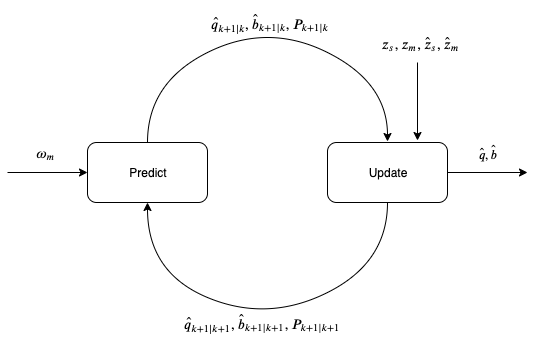
\includegraphics[width=0.7\linewidth]{ESKF.png}
    \end{figure}
\end{frame}

%------------------------------------------------

\begin{frame}
    \frametitle{ESKF code}
    \large{\centerline{Let's have a brief look at the code I guess?}}
   \begin{center}
    \small{Code: \url{https://git.orbitntnu.no/adcs/libeskf} \\
    Tests: \url{https://git.orbitntnu.no/adcs/eskf_test} \\
    Matlab tests: \url{https://git.orbitntnu.no/Martimos/adcs_simulation/tree/eskf-c-test}}
   \end{center}
\end{frame}

%------------------------------------------------

\begin{frame}
\huge{\centerline{Thank you for coming to my TEDx talk}}
\end{frame}

%----------------------------------------------------------------------------------------

\end{document} 